\subsubsection{Initial comparison - Default settings \label{sec:initialCompare}}
For the initial comparison we use the Bertsekas featureset, since the same featureset
was used for verifying the Cross Entropy implementation. Furthermore, others researchers
has used the Bertsekas featureset as a benchmarking standpoint \citep{thiery:09} \&
\citep{szita:06}.\\
The goal of this comparison is to get an initial idea of how the Shark implementation of
CMA-ES compares to the Cross-entropy method with settings used by other researchers \citep{thiery:09}.\\

\textbf{Results}

Using Cross-entropy method with the constant noise setting and CMA-ES with an initial step-size
of $0.5$, we get the following results, seen in figure \ref{fig:CMA_VS_CE_00}.\\

\begin{figure}[H]
\begin{center}
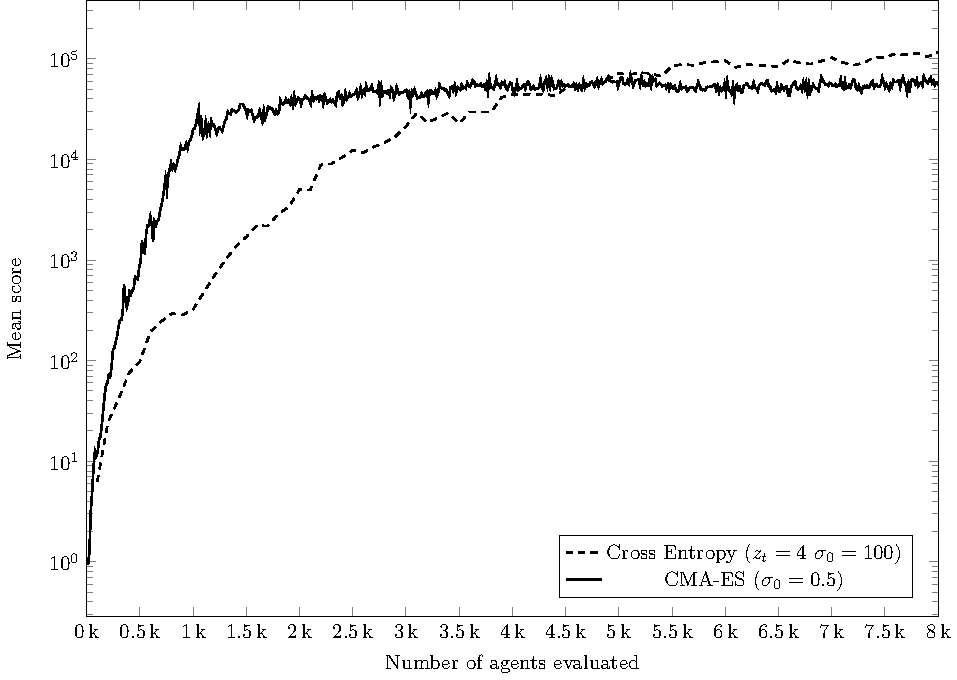
\includegraphics[scale=0.8]{plots/cmaCePlot}
\end{center}
\caption{Initial comparison between CMA-ES and Cross-entropy method \label{fig:CMA_VS_CE_00}}
\end{figure}

\begin{table}[H]
\centering
\small
\begin{tabular}{l r r r r}
Optimizer & Mean & Q1 & Q2 & Q3\\
\hline
CMA-ES  & $57783.0$ & $10269.9$ & $59774.5$ & $100384.1$\\
The Cross-entropy method & $116289.4$ & $85230.9$ & $125329.5$ & $138715.5$\\
\end{tabular}
\caption{Results from last iteration of the curves in figure \ref{fig:CMA_VS_CE_00}
\label{table:initialResultTable}}
\end{table}

As figure \ref{fig:CMA_VS_CE_00} reveals that CMA-ES converges faster,
but reaches a local optimum at around 2,000 games played. Meanwhile Cross-entropy method has a 
slower convergence but reaches a better mean score compared to CMA-ES at around 5,500
agents evaluated. In detail, CMA-ES on average reaches a score of 50,000 rows, and
Cross-entropy method reaches a score of 100,000.\\

\textbf{Analysis and discussion}

These results clearly defy our initial hypothesis as we predicted
for CMA-ES to outperform Cross-entropy method, due to its more sophisticated nature. 
One reason for this outcome could possibly be that
CMA-ES has a very little population size compared to Cross-entropy method,
which could be a decisive lack as the objective function is noisy with 
a high variance.\\

\comment{Remove rest of section because it is absolute from previous sections?}
Among the possible adjustments are:\\
\\
\textit{Enlargment of population size}\\
As the population size is quite small (only around 13)
for this experiment, the CMA-ES algorithm might not be able
extract enough information at each generation. As seen in 
section \ref{optimalsettingsce}, CE looses performance as 
the population size is set too low. This might be a problem 
that counts for CMA-ES as well. In figure \ref{fig:CMA_VS_CE_00},
the CMA-ES algorithm has much the same shape as \\
\\
\textit{Evaluate each agent multiple times}\\
A posible source of poor performance could be 
that the ranking of agents becomes very difficult
due to high noise. To better verify the actual
performance of an agent, it could be evaluated 
multiple times and let the mean of the evaluations
determine it's ranking.\\
\\
\textit{Change the recombination type}\\
As described in section \ref{CMAtheory}, 
the CMA-ES is not bound to update its 
new mean to just the centroid of the selected 
vectors. Instead, it can weight better solutions
more heavily when moving its mean. When doing so,
it risks biasing vectors that appear to be better 
but in reality, just by faulty ranking, should
not be considered a good agent.\\
\\
None of the experiments seen so far has allowed a 
consistent mean score of more 
than 200,000. This brings concern into 
consideration, that it might be the objective function
that poses a natural limit on the score.
In this case the objective function
models playing Tetris with the Bertsekas featureset. 
It is unkown to us
whether it's possible to construct an agent 
with a mean score of more than
200,000 lines on average. 
Yet, as our aim is not to find the best controller,
untill both algorithms reaches the same upper limit 
of scores theres is no need
to alter the featureset just to
expand the maximum score reachable.\\
\\
Yet, to minimize the likelihood 
that the featureset were the cause of the 
poor performance of CMA-ES, it seemed 
appropiate to conduct a similar comparison 
using another featureset. 
To speed up the process, the game difficulty were 
adujsted to casue agents to fail faster.
The increased difficulty and alternate
featureset is described in 
further detail in section \ref{compoffeatureset}.

